\documentclass{article}
\usepackage[left=25mm,right=25mm,bottom=35mm]{geometry}
\usepackage{amsmath,graphicx}
\usepackage[comma,numbers,square,sort&compress]{natbib}

\begin{document}

\title{Fault Diagnosis of Variable Pitch for Wind Turbines Based on Multi-innovation Forgetting Gradient Identification Algorithm}

\author{Dinghui WU,
        Yiyang LI}
\date{}
\maketitle



\begin{abstract}
This paper presents the fault diagnosis algorithm of variable pitch system for wind turbines. The considered variable pitch system model is characterized by second order differential equation, and then transformed into discretization equation and difference equation. We transform the fault diagnosis problem into a parameter estimation issue, and the multi-innovation forgetting gradient (MIFG) identification algorithm is adopted. Because the MIFG algorithm uses not only current data but also the past data at each iteration, the parameter estimation accuracy is improved. The validity of fault diagnosis using MIFG algorithm for pitch system is verified by simulation example.
\end{abstract}

%\keywords{Wind Turbine, System Identification, Pitch System, Fault Diagnosis, MIFG}



\footnotetext{\\
Key laboratory of Advanced Process Control for Light Industry, Ministry of Education, Jiangnan University, Wuxi, China\\
Corresponding author:\\
Dinghui Wu, Key laboratory of Advanced Process Control for Light Industry, Ministry of Education, Jiangnan University, Wuxi 214133, China\\
Email: wh033098@163.com}


\section{Introduction}

Today, wind energy has contributed to a large part of world power production\cite{ref:1}, and variable pitch system has played a important role in wind turbines. Since most wind turbines are located in remote areas, they are expected to produce energy with reliability and stability\cite{ref:2}. An effective way to ensure this is adopting advanced fault diagnosis technology, even though it may result in less power production in some cases\cite{ref:3}.

\begin{figure}[!htb]
  \centering
  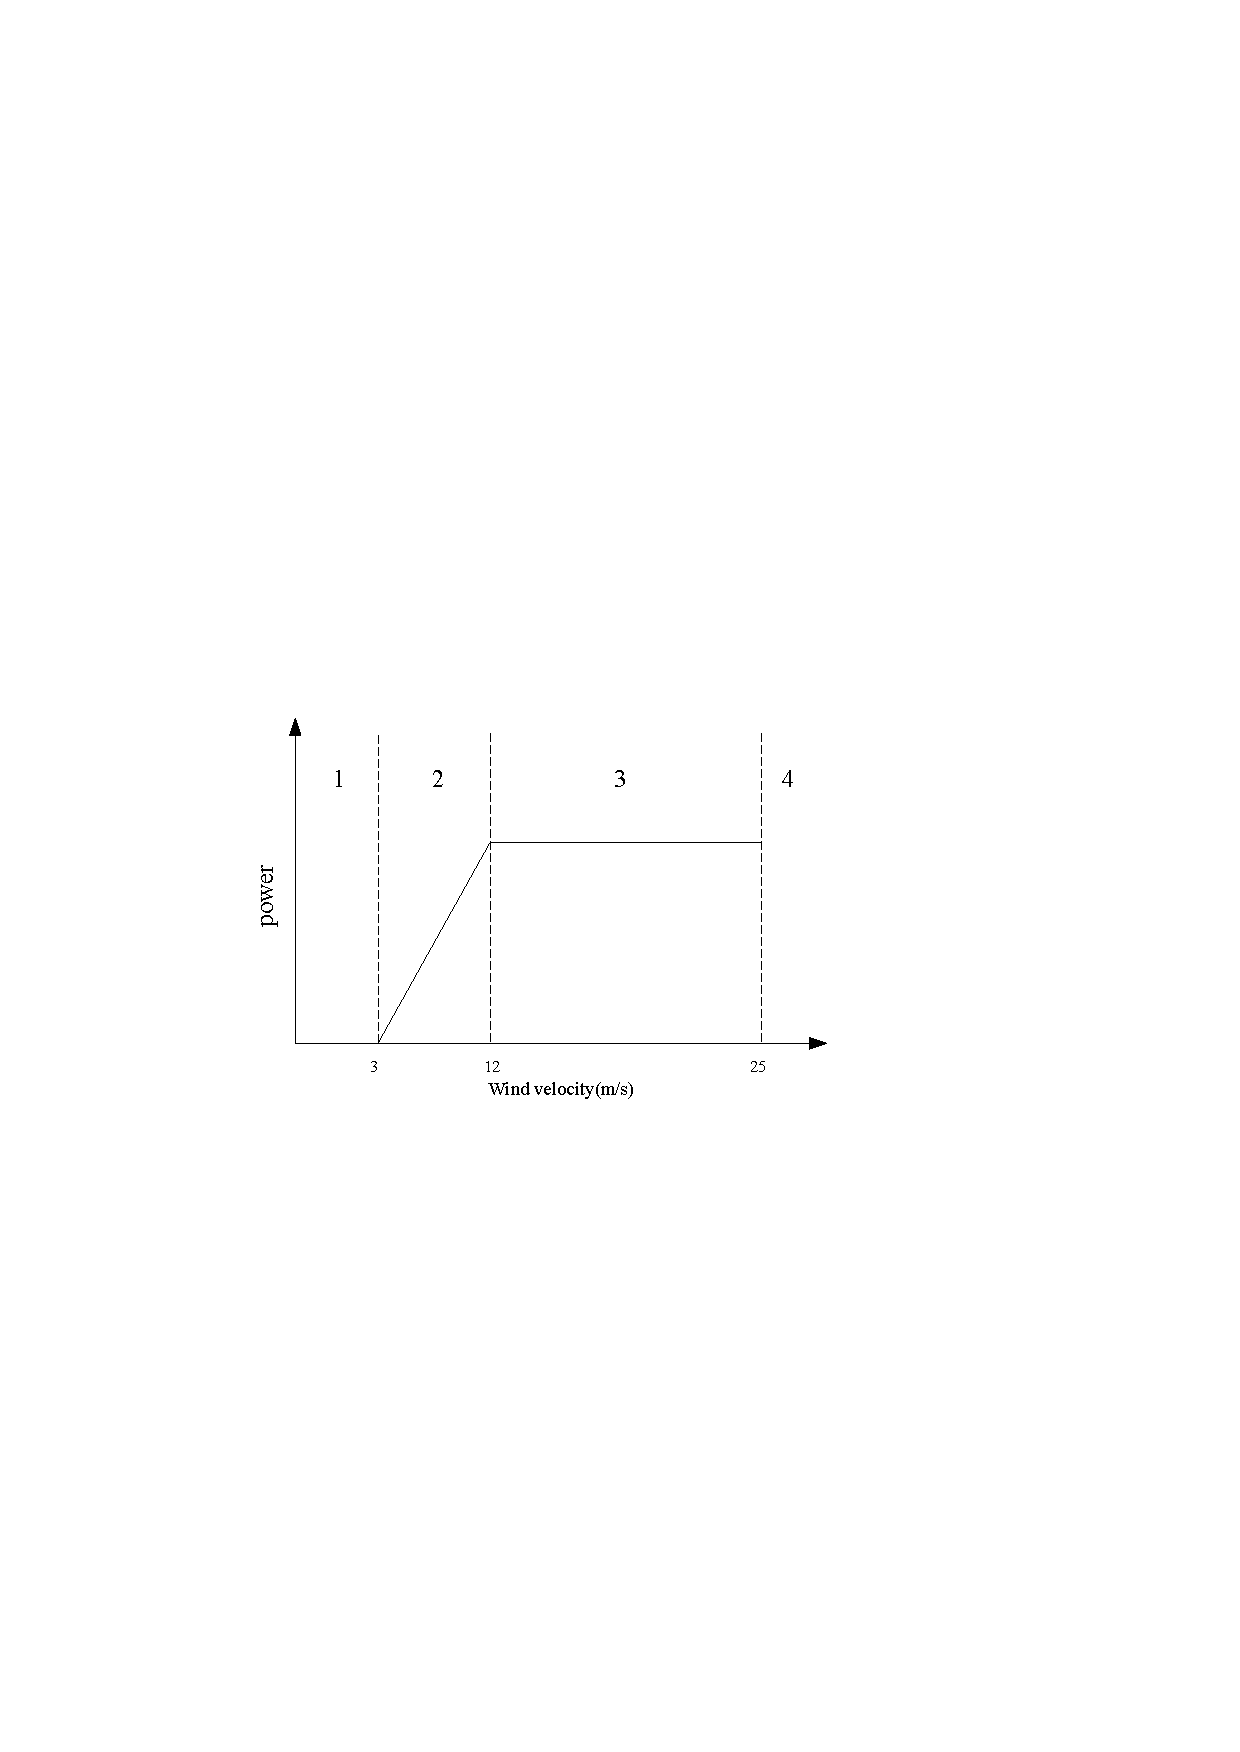
\includegraphics[width=\hsize]{Visio-four_zone.pdf}
  \caption{Four Operational Zones of Wind Turbine}
  \label{fig:1}
\end{figure}

The wind turbine operates in four operational zones governed by the mean wind velocity as depicted in Fig.\ref{fig:1}. In zone 1, the turbine is standstill; zone 2 is optimized to capture the maximum wind power; in zone 3, the pitch system works to keep constant power production; in zone 4, the wind velocity is too high and the wind turbine is kept shutdown\cite{ref:wind zone}. The hydraulic pitch system fault directly affects the production stability when the turbine is in zone 3. At present, fault diagnosis researches of hydraulic variable pitch system for wind turbine are mainly as follows. In \cite{ref:neural BP}, Wang has studied to carry on fault diagnosis of pressure with integration BP neural network theory.
% 2013.9.25
Wang's method is effective for the non-linear dynamic process in hydraulic system, but BP neural network theory still lacks proof and is difficult to obtain the estimation error bound.
% 2013.9.25 remove peti's method, add wavelet method
In \cite{ref:qualitative pitch}, Goharrizi analyzes the pressure signal at one side of the actuator in response to periodic step inputs to the control valve. It is shown that with discrete wavelet transform (WT), detail version of pressure signal can be obtained to detect internal leakage and its severity. The only disadvantage is that the method can only work offline, which limits the use.
%
In \cite{ref:active LPV}, Sloth uses extended kalman filter to estimate the tower acceleration caused by pitch system, by comparing the estimated acceleration value using fault data with true tower acceleration sensor value, Sloth's study is able to determine which pitch is uncontrollable and the degree of the fault.
% 2013.9.25
But Sloth's method relies a lot on past data, which increase the burden of the processor. Also, this method uses the tower acceleration sensor, which is not available in some kinds of wind turbines.
%%%%%%%%%
%% 2013.9.24 begin
%%%%%%%%%
% add some description about the disadvantages of conventional diagnosis
%%%%%%%%%
%% 2013.9.25 end
%%%%%%%%%

System identification is one of the major research fields of modern control theory\cite{ref:ding1}. A lot of identification methods have been proved to have minimum estimation error\cite{ref:ding2}, identifiability\cite{ref:ding3} and be identified online\cite{ref:ding4}.
In this paper, we try to convert the fault diagnosis problem into a system identification issue. The following faults may happen to pitch system, they are: pump wear, hydraulic leakage, high air content in the hydraulic oil\cite{ref:active LPV}. These faults change the dynamics of the pitch system and make the system uncontrollable. In system identification view, the pitch system with fault can be modeled as a time-varying system. An effective way to estimate the time-varying system is within the framework of identification algorithm with a forgetting factor $\lambda$.
%%%%%%%%%
%% 2013.9.25 begin
%%%%%%%%%
% add some description about system identification
%%%%%%%%%
%% 2013.9.25 end
%%%%%%%%%

A few work has been done to deal with time-varying system's parameter estimation. In 1995, Guo and Ljung studied the estimation error of recursive least squares (RLS) with a forgetting factor (RFFLS for short)\cite{ref:rls}, they assumed that the error $v(t)$ and parameter drift $w(t)$ can be modeled as white noise. In \cite{ref:rffls}\cite{ref:misg}, Ding studied the detail of RFFLS's estimation error bounds and prove only in deterministic systems, the algorithm is exponentially convergent.



The rest of the paper is organized as follows. Section 2 gives wind turbine model for simulation and the differential equation model of pitch system. And then utilizing a new way to convert it into a difference equation model. In Section 3, the algorithm's procedure and analysis of MIFG is given, which mainly focuses on how to choose the forgetting factor $\lambda$. Section 4 contains a simulation result and followed by the conclusion in Section 5.


%%%%%%%%%
%% 2013.9.25 begin
%%%%%%%%%
% add wind turbine model
%%%%%%%%%
%% 2013.9.26 end
%%%%%%%%%
\section{Wind Turbine Model}

In order to establish the simulation model, the whole wind turbine model should be analyzed, even though the identification algorithm focuses on the pitch system. The turbine is composed of aerodynamics, pitch, drive train and generator convertor\cite{ref:lyy1}.

\subsection{Wind Turbine Model Excluding Pitch}

The pitch converts the energy from wind to rotor shaft, the shaft rotates at the speed $\omega_r(t)$, the wind power is dependent on wind velocity $v_r(t)$, air density $\rho$ and the rotate area $A$. The converted wind power is based on power coefficient $C_p(\lambda(t), \beta(t))$, where $\lambda(t)$ is tip-speed ratio and $\beta(t)$ is pitch angle. The aerodynamic torque applied on rotor shaft is given as\cite{ref:robust1}:

\begin{equation}
  T_a(t) = \frac{1}{2\omega_r(t)}\rho{}Av^3_r(t)C_p(\lambda(t),\beta(t))
\end{equation}

The drive train is consisted of low-speed shaft and high-speed shaft, the inertias and friction coefficient of both side are $J_r, J_g$ and $B_r, B_g$. The two shafts are interconnected by gears, and the gear ratio is $N_g$, combined with torsion stiffness $K_{dt}$ and torsion damping $B_{dt}$. This results in a torque applied to generator $T_g(t)$ with a speed $\omega_g(t)$. The drive train model is given as\cite{ref:robust2}:
\begin{eqnarray}
  J_r\dot{\omega_r}(t) &= T_a(t) + \frac{B_{dt}}{N_g}\omega_g(t) \notag\\
  & -(B_{dt} + B_r)\omega_r(t) \\
  J_g\dot{\omega_g}(t) &= \frac{B_{dt}}{N_g}\omega_r(t) - T_g(t) \notag \\
  & -(\frac{B_{dt}}{N^2_g} + B_g)\omega_g(t)
\end{eqnarray}

Electric power is generated by the generator, while the generator torque is adjusted by the reference $T_{g,ref}(t)$. The actual torque from converter is described as a first order system with time constant $\tau_g$ and time delay $t_{g,d}$\cite{ref:active LPV}.
\begin{equation}
  \dot{T_g}(t) = -\frac{1}{\tau_g}T_g(t) + \frac{1}{\tau_g}T_{g,ref}(t-t_{g,d})
\end{equation}

The electric power produced by the generator is described as follows, where the $\eta$ is efficiency of generator, which is considered to be a constant\cite{ref:active LPV}.
\begin{equation}
  P_g(t) = \eta_g\omega_g(t)T_g(t)
\end{equation}
%%%%%%%%%
%% 2013.9.25 begin
%%%%%%%%%
% add wind turbine model
%%%%%%%%%
%% 2013.9.26 end
%%%%%%%%%


\subsection{Pitch System Model Including Fault Model}

The purpose of this section is to explain how the pitch system is modeled. The pitch system shown in Fig.\ref{fig:2} ajusts the pitch of a blade by rotating it according to wind velocity. In general, one turbine is composed of three pitches, each pitch is regulated by a hydraulic actuator, which are controlled separately by three valves.

\begin{figure}[!htb]
  \centering
  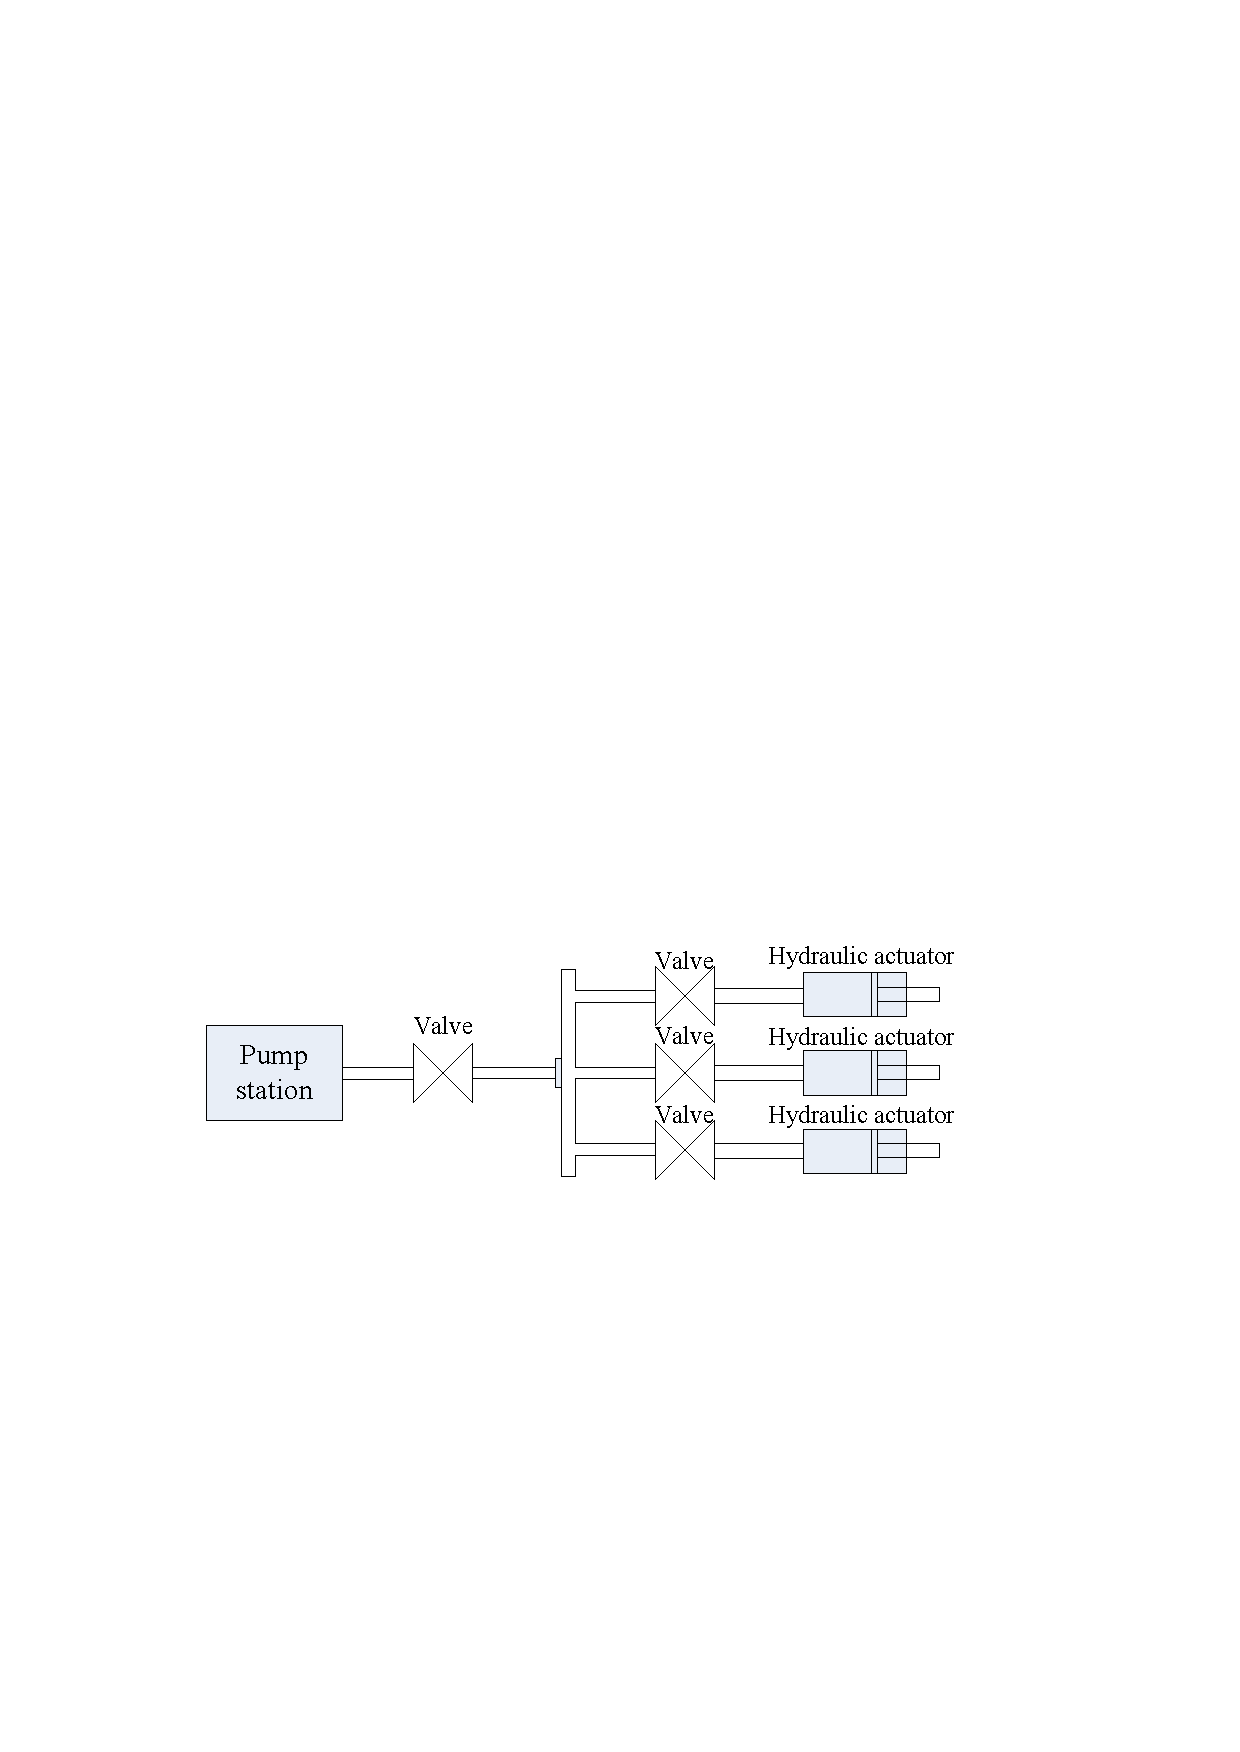
\includegraphics[width=\hsize]{Visio-pitchsystem.pdf}
  \caption{Hydaulic Pitch System}
  \label{fig:2}
\end{figure}


The hydraulic pitch is modeled as a second order system, described as:

\begin{eqnarray}\label{e:1}
\frac{\beta(s)}{\beta_{ref}(s)} &=& \frac{\omega^2_n}{s^2 + 2\zeta\omega_n{}s+\omega_n^2} \\
\ddot{\beta}(t) &=& -2\zeta\omega_n\dot{\beta}(t) - \omega^2_n\beta(t) + \omega^2_n\beta(t) + \omega^2_n\beta_{ref}(t) \notag
\end{eqnarray}
where: \\
$\beta(t)$ is the pitch angle,\\
$\beta_{ref}(t)$ is the reference to the pitch angle,\\
$\omega_n$ is the natural frequency of the pitch model, \\
$\zeta$ is the damping ratio of the pitch model

Since the algorithm will finally be ported to a computer or some embedded processor, it is necessary to change the Eq.\ref{e:1} into the difference one. There are many conventional ways to transform the Laplace equation, like bilinear transform and Euler transform, but these methods are simple and will lose accuracy during transformation, which is difficult to meet the industrial requirements.

From the given plant $G(s)$ and sampling period $T$, we can obtain the only linearization model $G(z)$ using a new method called impulse invariance transformation\cite{ref:ding5}, which can gurantee the accuracy during transformation from continuous linear model to discrete model.

First, we denote
\begin{eqnarray*}
a &:=& -2\zeta\omega_n+\frac{\sqrt{4\zeta^2\omega^2_n-4\omega_n^2}}{2}\\
b &:=& -2\zeta\omega_n-\frac{\sqrt{4\zeta^2\omega^2_n-4\omega_n^2}}{2}\\
G(s) &:=& \frac{\beta(s)}{\beta_{ref}(s)} = \frac{ab}{s^2+(a+b)s+ab}
\end{eqnarray*}
then, using the impulse invariance transformation, the discrete equation is:
\begin{eqnarray}
  G(z) &=& \frac{1}{2\pi{}j}\oint_c G(s) \frac{z}{z-e^{Ts}}ds \notag\\
        &=& \frac{1}{2\pi{j}}\oint_c\frac{ab}{(s+a)(s+b)}\frac{1}{1-e^{Ts}z^{-1}}ds \notag \\
        &=& \frac{1}{b-a}\frac{ab(e^{-aT}-e^{-bT})z^{-1}}
        {1 - (e^{-aT}+e^{-bT})z^{-1} + e^{-(a+b)T}z^{-2}} \notag \\
\end{eqnarray}
then, the difference equation can be obtained:
\begin{eqnarray}
  &G(z) = y(t)/u(t) \notag \\
  &(b-a)[1 - (e^{-aT}+e^{-bT})z^{-1} + e^{-(a+b)T}z^{-2}]y(t) \notag \\
  &= [ab(e^{-aT}-e^{-bT})z^{-1}]u(t) \notag \\
\end{eqnarray}
finally:
\begin{eqnarray}
y(t) - (e^{-aT}+e^{-bT})y(t-1) + e^{-(a+b)T}y(t-2) \notag \\
= \frac{ab}{b-a}(e^{-aT}-e^{-bT})u(t-1)
\end{eqnarray}
the identification model can be expressed as:
\begin{eqnarray} \label{e:time-varying}
  y(t) = \varphi^\mathrm{T}\theta(t) + v(t)
\end{eqnarray}
where \\
$\theta(t):=[- (e^{-aT}+e^{-bT}), e^{-(a+b)T}, \frac{ab}{b-a}(e^{-aT}-e^{-bT})]^\mathrm{T}$, \\ $\varphi(t):=[y(t-1), y(t-2),u(t-1)]^\mathrm{T}$ ,\\
$v(t)$ is the zero mean white noise.

The faults considered for pitch system are: pump wear, hydraulic leakage, high air content. They can be modeled as follows.
\begin{eqnarray}
  \tilde{\zeta}(t) &=& (1-\alpha_{pw}(t))\zeta + \alpha_{pw}(t)\zeta_{pw} \notag \\
  \tilde{\omega}_n(t) &=& (1-\alpha_{pw}(t))\omega_n + \alpha_{pw}(t)\omega_{n,pw} \\
  \tilde{\zeta}(t) &=& (1-\alpha_{hl}(t))\zeta + \alpha_{hl}(t)\zeta_{hl} \notag \\
  \tilde{\omega}_n(t) &=& (1-\alpha_{hl}(t))\omega_n + \alpha_{hl}(t)\omega_{n,hl} \\
  \tilde{\zeta}(t) &=& (1-\alpha_{ha}(t))\zeta + \alpha_{ha}(t)\zeta_{ha} \notag \\
  \tilde{\omega}_n(t) &=& (1-\alpha_{ha}(t))\omega_n + \alpha_{ha}(t)\omega_{n,ha}
\end{eqnarray}
where \\
$\alpha_{pw}$ is an indicator for the pump wear, \\
$\alpha_{hl}$ is an indicator for the hydraulic leakage, \\
$\alpha_{ha}$ is an indicator for the high air content in oil.

The parameters for the above three faults are shown in the table.

\begin{table}[!htb]
  \centering
  \caption{Parameters' Value}
\begin{tabular}{|c|c|}
  \hline
  % after \\: \hline or \cline{col1-col2} \cline{col3-col4} ...
  Fault & Parameters \\\hline\hline
  No Fault & $\omega_n=11.11rad/s$, \\
            &       $\zeta=0.6$        \\\hline
  Pump Wear & $\omega_{n,pw}=7.27rad/s$,\\
            &       $\zeta_{pw}=0.75$    \\\hline
  Hydraulic Leakage & $\omega_{n,hl}=3.42rad/s$, \\
            &   $\zeta_{n,hl}=0.9$        \\\hline
  High Air Content  & $\omega_{n,ha}=5.73rad/s$, \\
       in the Oil     &   $\zeta_{n,ha}=0.45$ \\
  \hline
\end{tabular}
\end{table}

%%%%%%%%%
%% 2013.9.26 begin
%%%%%%%%%
% add assembled model
%%%%%%%%%
%% 2013.9.26 end
%%%%%%%%%
\subsection{Assembled Model}

The sub-models are connected as depicted in Fig.\ref{fig:assembled}. The system is sampled at a rate of $T=100Hz $.

\begin{figure}[!htb]
  \centering
  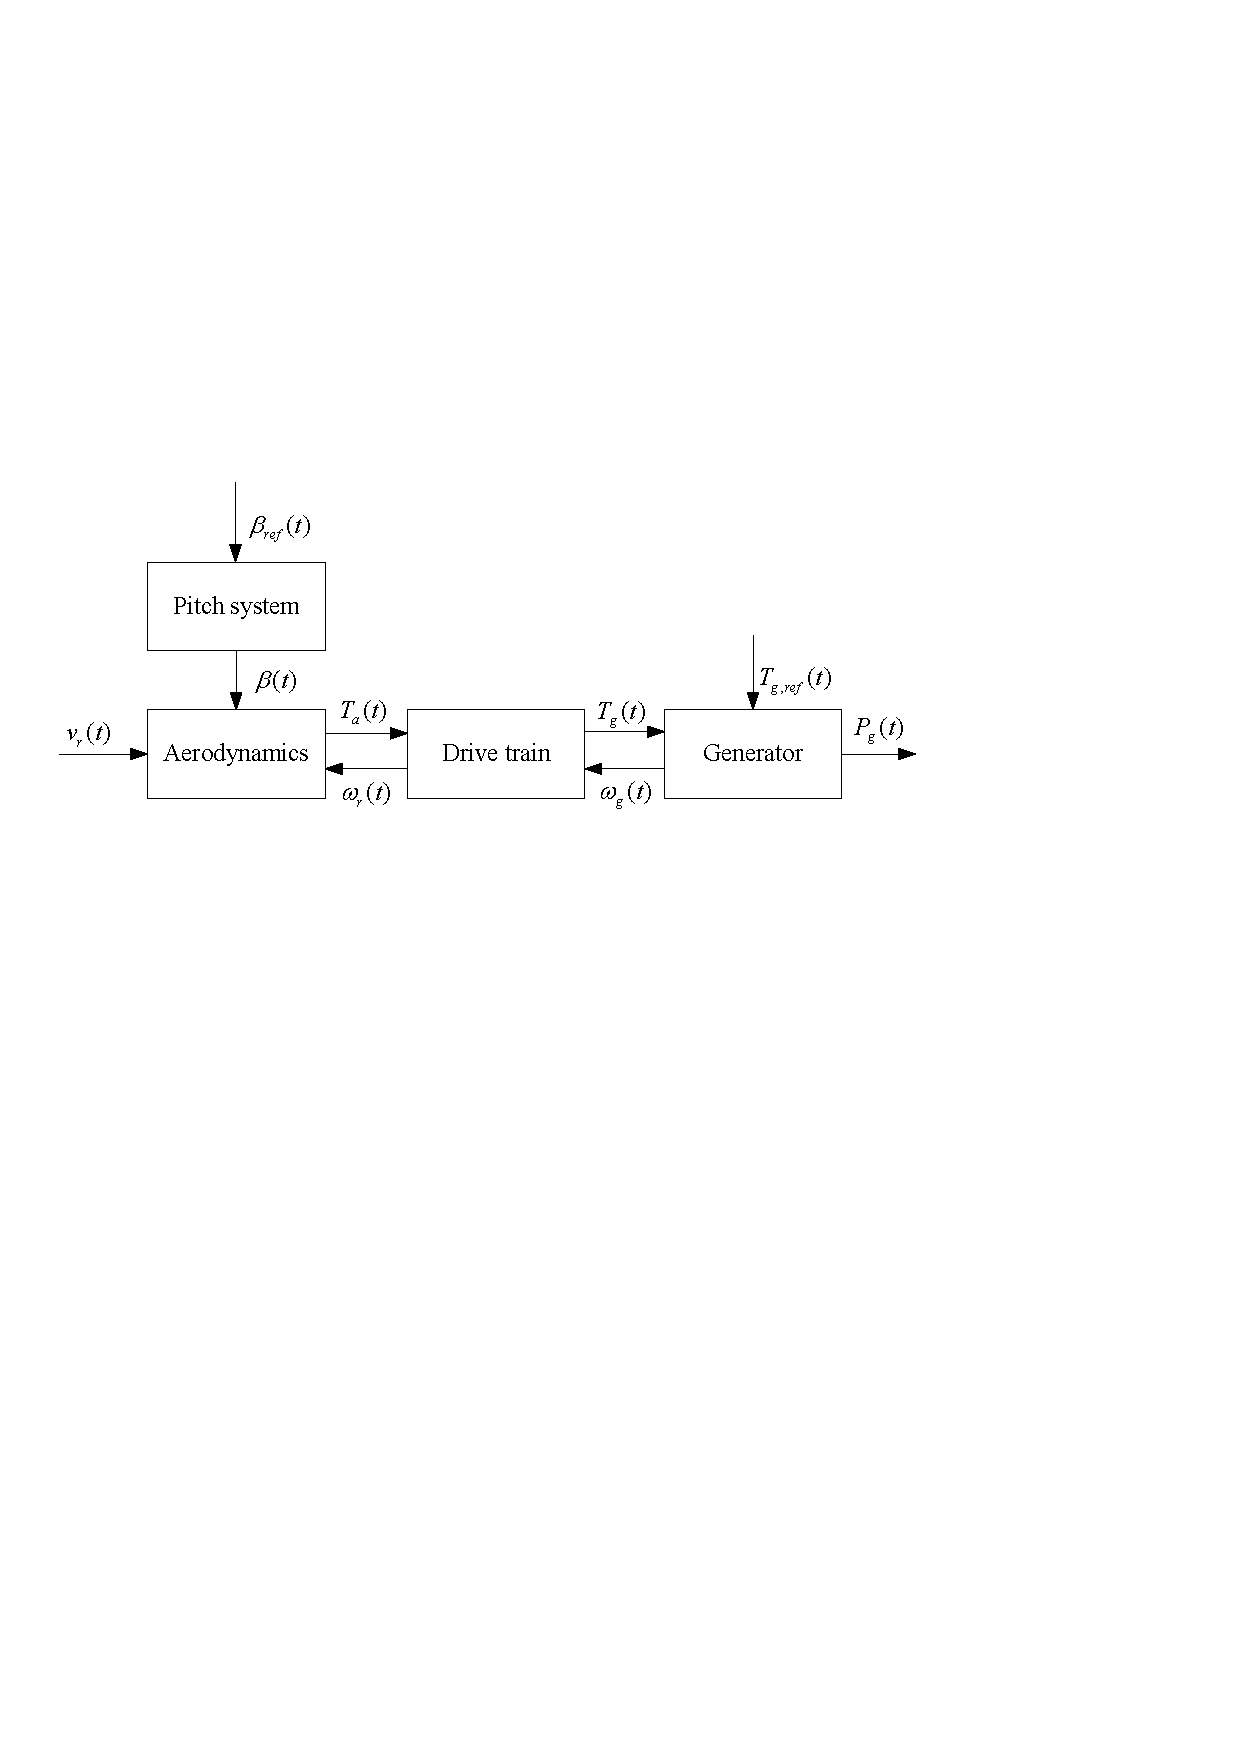
\includegraphics[width=\hsize]{Visio-assembled1.pdf}
  \caption{Structure of Pitch System}
  \label{fig:assembled}
\end{figure}



%%%%%%%%%
%% 2013.9.26 begin
%%%%%%%%%
% add algorithm description
%%%%%%%%%
%% 2013.9.27 end
%%%%%%%%%
\section{Description of Fault Diagnosis algorithm}

In this section, we give the procedure to implement the fault diagnosis system, and present a short discussion on how to choose the forgetting factor $\lambda$ to obtain the minimum estimation error.

\subsection{structure of Fault Diagnosis algorithm}

Fig.\ref{fig:assembled} shows the wind turbine structure, the fault diagnosis based on system identification needs the pitch system's input and output. We take the pitch controller's output $\beta_{ref}(t)$ as input, and the actual pitch angle $\beta(t)$ as output. The reformed structure is shown below.

\begin{figure}[!htb]
  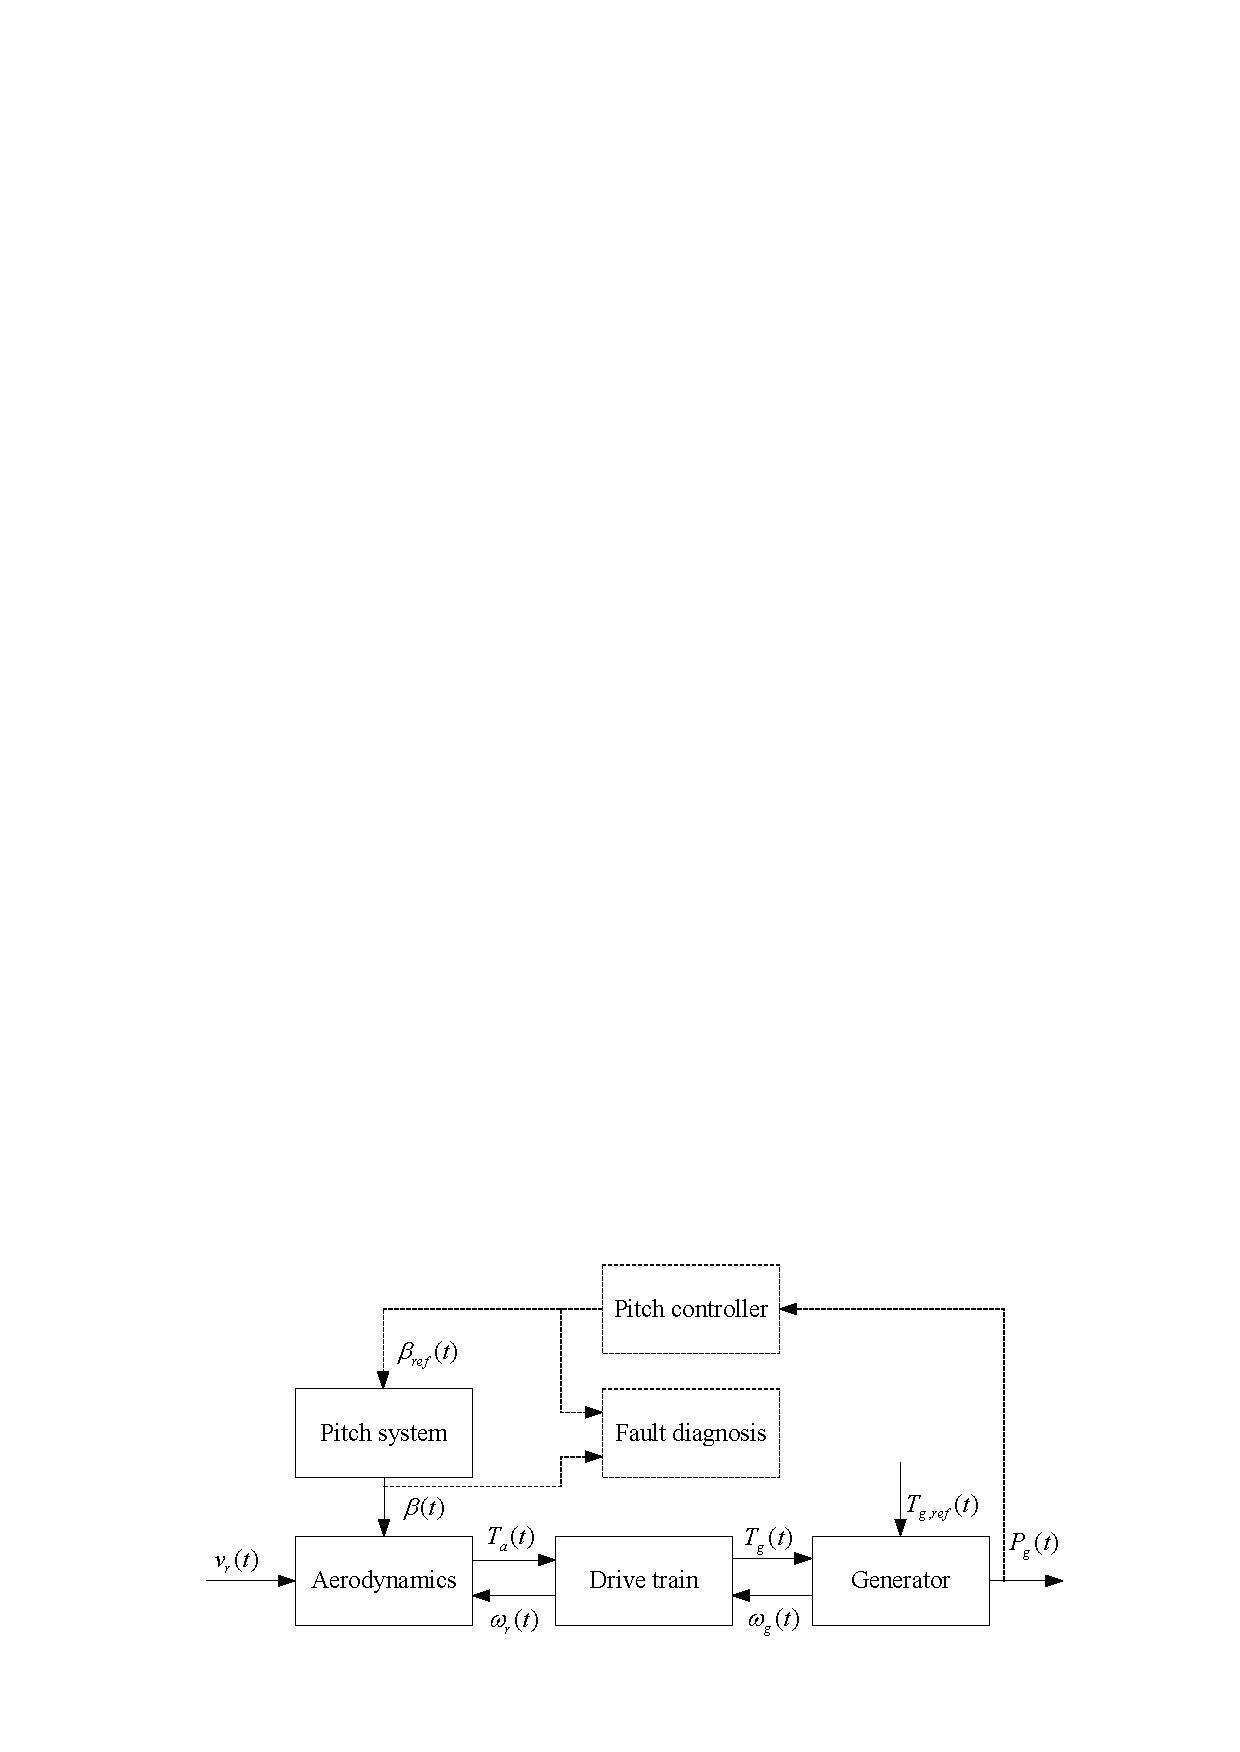
\includegraphics[width=\hsize]{Visio-assembled2.pdf}
  \caption{Simulation Structure}
  \label{fig:assembled_diagnosis}
\end{figure}

As the wind turbine in our paper operates in zone 3, the pitch controller is designed by taking the electric power as input and pitch reference $\beta_{ref}$ as output, which will maintain the generated power constant despite of the disturbance input $v_r(t)$.
%%%%%%%%%
%% 2013.9.26 begin
%%%%%%%%%
% add algorithm description
%%%%%%%%%
%% 2013.9.27 end
%%%%%%%%%

\subsection{Analysis of MIFG}

Innovation is defined as useful information which can improve parameter estimation accuracy\cite{ref:dinf6}. Consider the least square and gradient stochastic algorithms, the identification system is:
\begin{equation}
  y(t) = \varphi^\mathrm{T}(t)\theta + v(t)
\end{equation}
where, $y(t)\in{}R$ is output, $\theta(t)\in{}R^n$ is parameter vector to be identified, $\varphi\in{}R^n$ is the information vector consisting of the system input-output data, $v(t)$ is the stochastic noise with zero mean. The general identification algorithm is:
\begin{equation}
  \hat{\theta}(t) = \hat{\theta}(t-1) + L(t)e(t)
\end{equation}
where $L(t)\in{}R^n$ is gain vector, $e(t):=y(t)-\varphi^\mathrm{T}(t)\hat{\theta}(t-1)\in{}R$ is scalar innovation, that is single innovation.

We extend the single innovation to multi-innovation, which means that \\
$E(p,t)=\begin{bmatrix}
  e(t)\\
  e(t-1)\\
  \vdots \\
  e(t-p+1)
\end{bmatrix}\in{}R^p$, $p$ is the innovation length.

By defining the information matrix $\Phi(p,t)$ and stacked output vector $Y(p,t)$ as\\
$\Phi(p,t)=[\varphi(t),\varphi(t-1),...,\varphi(t-p+1)]\in{}R^{n\times{}p}$,\\
$Y(p,t)=[y(t),y(t-1),...,y(t-p+1)]^{\mathrm{T}}\in{}R^p$,\\
the innovation vector $E(p,t)$ may be expressed as\\
$E(p,t)=Y(p,t) - \Phi^{\mathrm{T}}(p,t)\hat{\theta}(t-1)$.


The least square identification algorithm converges fast, but will suffer from high computation due to covariance matrix. gradient stochastic identification algorithm has a small mount of computation, but converges really slow. Both types of algorithm is not suitable in wind turbine system. By applying the multi-innovation into gradient stochastic algorithm, we will have a new algorithm which can compute quickly and converge fast. In order to track a time-varying system, we also apply a forgetting factor $\lambda$, that is MIFG algorithm.

\subsection{How to Choose Forgetting Factor and Innovation Length}

The purpose of this subsection is to give short discussion on how to choose $\lambda$ and $p$.
Consider the time-varying system \ref{e:time-varying}, where $\theta(t)\in{}R^n$ is the time-varying parameter vector to be identified.

The MIFG algorithm of estimating $\theta(t)$ may be expressed as :
\begin{eqnarray}
  \hat{\theta}(t) &=& \hat{\theta}(t-1) + \frac{\Phi(t)}{r(t)}[Y(t) - \Phi^\mathrm{T}\theta(t-1)], \label{e:mifg1} \\
  r(t) &=& \lambda{}r(t-1)  + \|\varphi(t)\|^2, 0<\lambda<1, r(0)>0, \label{e:mifg2} \notag\\
  \\
  \Phi(p,t) &=& [\varphi(t), \varphi(t-1), \ldots, \varphi(t-p+1)]\in{}R^{n\times{}p}, \label{e:mifg3} \notag\\
  \\
  Y(p,t) &=& [y(t), y(t-1), \ldots, y(t-p+1)]^{\mathrm{T}}\in{}R^p. \label{e:mifg4} \notag\\
\end{eqnarray}

In engineering, the parameter estimation accuracy is meassured by $\delta_a := \|\hat{\theta}(t) - \theta(t)\|^2$, but as the parameter vector $\theta(t)$ is unknown, it is impossible to obtain $\delta_a$. It is necessary for us to analyze the upper bound of estimation error, and can be simplified as Theorem 1.

Here, we assume that the information vector $\varphi(t)$ is persistently exciting, that is, there exist constants $0<\alpha\leq\beta<\infty$ and an integer $N\geq{}n$ such that the following persistent excitation condition holds\cite{ref:ding1}:
\begin{equation}
  \alpha{}I \leq \frac{1}{N}\sum^{N-1}_{i=0}\varphi(t+i)\varphi^\mathrm{T}(t+i)\leq \beta{}I , t>0.
\end{equation}

For the system Eq.\ref{e:time-varying} and the MIFG algorithm in Eq.\ref{e:mifg1}-Eq.\ref{e:mifg4}, $r(0)$ is chosen by $\frac{\alpha}{1-\lambda}\leq{}r(0)\leq\frac{nN\beta}{1-\lambda}$, let the innovation length $p=N$ and $E[\|\hat{\theta}(0) - \theta(0)\|^2] = \delta_0 < \infty$, the observation noise $\{v(t)\}$ and the parameter changing rate ${w(t):=\theta(t)-\theta(t-1)}$ are stochastic sequences with zero mean, and the sequences $\{v(t)\}$ and $\{w(t)\}$ satisfy
\begin{eqnarray}
  E[v(t)]=0, E[w(t)]=0, \\
  E[v^2(t)]\leq\sigma^2_v<\infty, E[\|w(t)\|^2] \leq^2_w < \infty.
\end{eqnarray}

Next, we define the noise vectors as following: ����
$w(t)=\theta(t)-\theta(t-1)$, we can define the noise vector, \\
$V(p,t) :=
\begin{bmatrix}
  v(t)\\
  t(t-1)\\
  \vdots \\
  v(t-p+1)
\end{bmatrix}\in R^p,$\\
$W(p,t):=
\begin{bmatrix}
  0 \\
  \varphi^\mathrm{T}(t-1)w(t-1) \\
  \varphi^\mathrm{T}(t-2)[w(t-1)+w(t-2)] \\
  \vdots \\
  \varphi^\mathrm{T}(t-p+1)\sum^{p-1}_{j=1}w(t-j)
\end{bmatrix}\in{}R^p
$\\
and the parameter estimation error vector $\hat{\theta}(t)-\theta(t)$ is denoted as $\tilde{\theta}(t)$, and by applying Eq.\ref{e:mifg1}:
\begin{eqnarray}
  \tilde{\theta}(t) &=& \hat{\theta}(t)-[\theta(t-1) + w(t)] \notag \\
  &=& [I-\frac{\Phi(p,t)\Phi^\mathrm{T}}{r(t)}] \tilde{\theta}(t-1) \notag\\
  && +\frac{\Phi(p,t)[-W(p,t)+V(p,t)]}{r(t)}-w(t). \label{e:estimation error} \notag \\
\end{eqnarray}
as the expectation \\
\begin{eqnarray}
  E[\|\Phi(p,t)V(p,t)\|^2] &\leq& p^2\beta\sigma^2_v, \notag \\
  &=&  N^2\beta\sigma^2_v
  \leq \frac{N^2\beta(1-\lambda)^2\sigma^2_v}{\alpha^2} \notag \\
  E[\|\Phi(p,t)W(p,t)\|^2] &\leq& \frac{(p-1)p^3\beta^2\sigma^2_w}{2} \leq \frac{p^4\beta^2\sigma^2_w}{2} \notag \\
  &=& \frac{N^4\beta^2\sigma^2_w}{2}
  \leq \frac{N^4\beta^2(1-\lambda)^2\sigma^2_w}{2\alpha^2} \label{e:noise} \notag \\
\end{eqnarray}
and
\begin{eqnarray}
  I-\frac{\Phi(p,t)\Phi^T(p,t)}{r(t)} &\leq& [1-\frac{\alpha(1-\lambda)}{n\beta}]I \notag\\
  &=& (1-\rho)I
\end{eqnarray}

By taking norm and expectation of both side of Eq.\ref{e:estimation error} and using the inequality $\|x+y\|^2\leq(1+a)\|x\|^2+(1+a^{-1}\|y\|^2), (a>0)$, we can obtain:
\begin{eqnarray}
  E\|\tilde{\theta}(t)\|^2 &\leq& (1+a)(1-\rho)E[\|\hat{\theta}(t-1)\|^2] + \notag\\
   && 3(1+a^{-1})[\frac{N^4\beta^2(1-\lambda)^2\sigma^2_w}{2\alpha^2} + \notag \\
   &&   \frac{N^2\beta(1-\lambda^2)\sigma^2_v}{\alpha^2} + \sigma^2_w] \label{e:esti expecta}
\end{eqnarray}
We take $a$ to satisfy $0<a<\frac{\rho}{1-\rho}$, that is $0<(1+a)(1-\rho)<1$, then the expectation Eq.\ref{e:esti expecta} turns into
\begin{eqnarray}
  E[\|\tilde{\theta}(t)\|^2] &\leq& [(1+a)(1-\rho)]^t{}E[\|\tilde{\theta}(0)\|^2] +\notag \\
  &&  \frac{3(1+a^{-1})}{1-(1+a)(1-\rho)}[\frac{N^4\beta^2(1-\lambda)^2\sigma^2_w}{2\alpha^2} +\notag \\
  &&  \frac{N^2\beta(1-\lambda)^2\sigma^2_v}{\alpha^2} + \sigma^2_w] \notag \\
  &\leq& [(1+a)(1-\rho)]^t\sigma_0 + \notag\\
  && \frac{3(1+a^{-1})}{1-(1+a)(1-\rho)}[\frac{N^4\beta^2(1-\lambda)^2\sigma^2_w}{2\alpha^2} + \notag \\
  && \frac{N^2\beta(1-\lambda)^2\sigma^2_v}{\alpha^2} + \sigma^2_w]  \label{e:upperbound1}
\end{eqnarray}
and we can denote
\begin{eqnarray}
  [\frac{N^4\beta^2(1-\lambda)^2\sigma^2_w}{2\alpha^2} + \frac{N^2\beta(1-\lambda)^2\sigma^2_v}{\alpha^2} + \sigma^2_w] &:=& f(\lambda) \notag \\
  \frac{3(1+a^{-1})}{1-(1+a)(1-\rho)} &:=& g(a) \notag \\
\end{eqnarray}
To get the upper bound of the estimation error, we must minimize the right hand side of the Eq.\ref{e:upperbound1}, let:
\begin{equation}
  \frac{dg(a)}{da}=0
\end{equation}
and as we define a to be positive, we can obtain the best value $a_0=\frac{1}{\sqrt{1-\rho}}-1$ ,
and the correspond minimum $g_{min}$ is
$$\frac{3}{(1-\sqrt{1-\rho})^2}$$
and the minimum upper bound can be expressed as
$$[\sqrt{1-\rho}]^t\delta_0 + g_{min}f(\lambda)$$
Since $[\sqrt{1-\rho}]^t\sigma_0$ is very small, we can omit it.  To get the minimum $f_{min}$, just let:
\begin{eqnarray}\label{e:f}
  \frac{df(\lambda)}{\lambda}&=&0
\end{eqnarray}
Eq.\ref{e:f} is a four-order equation, and generally has four solution to get the best forgetting factor.

From the above analysis, we conclude the following guide to choose the best forgetting factor:
\begin{itemize}
  \item if parameter $\rho$ is small, it will generate small estimation error upper bound, which means $\alpha$ and $\beta$ should be close enough,
  \item from Eq.\ref{e:noise}, the system noise should be as small as possible to get a small estimation error bound,
  \item also from Eq.\ref{e:f}, a small innovation length $N$ will produce small estimation error upper bound.
\end{itemize}


\section{Simulation}

In this section,  we test the MIFG algorithm in $Matlab/Simulink$ with the model constructed in Section 2 and algorithm described in Section 3. Our identification model is Eq.\ref{e:time-varying}. The wind turbine operational parameters are shown in the following.

\begin{table}[!htb]
  \centering
  \caption{Parameter Value} \label{tab:turbine parameter}
\begin{tabular}{c|c|c|c}
    \hline
    Parameter        &     Value        &  Parameter     & Value \\ \hline
    $N_g$    & $95$  & $B_r$     & $27.8Nm/(rad/s)$ \\ \hline
    $A$         & $10387m^2$    & $B_{dt}$  & $945kNm/(rad/s)$ \\ \hline
    $\rho$      & $1.225kg/m^3$ & $B_g$     & $3.034Nm/(rad/s)$ \\ \hline
    $J_r$       & $55\times10^6kgm^2$ & $J_g$       & $390kgm^2$  \\ \hline
\end{tabular}
\end{table}

The pitch controller described in Fig.\ref{fig:assembled_diagnosis} is implemented as a PI controller, the detailed simulation structure is shown below. The electric power $P_g$ is the controller input, and the $\beta_{ref}$ is the controller output. Although there is more complex and better controller, but for simulation convenience, we choose the simplest PI controller, where $K_p=4, K_i=1$.

\begin{figure}[!htb]
  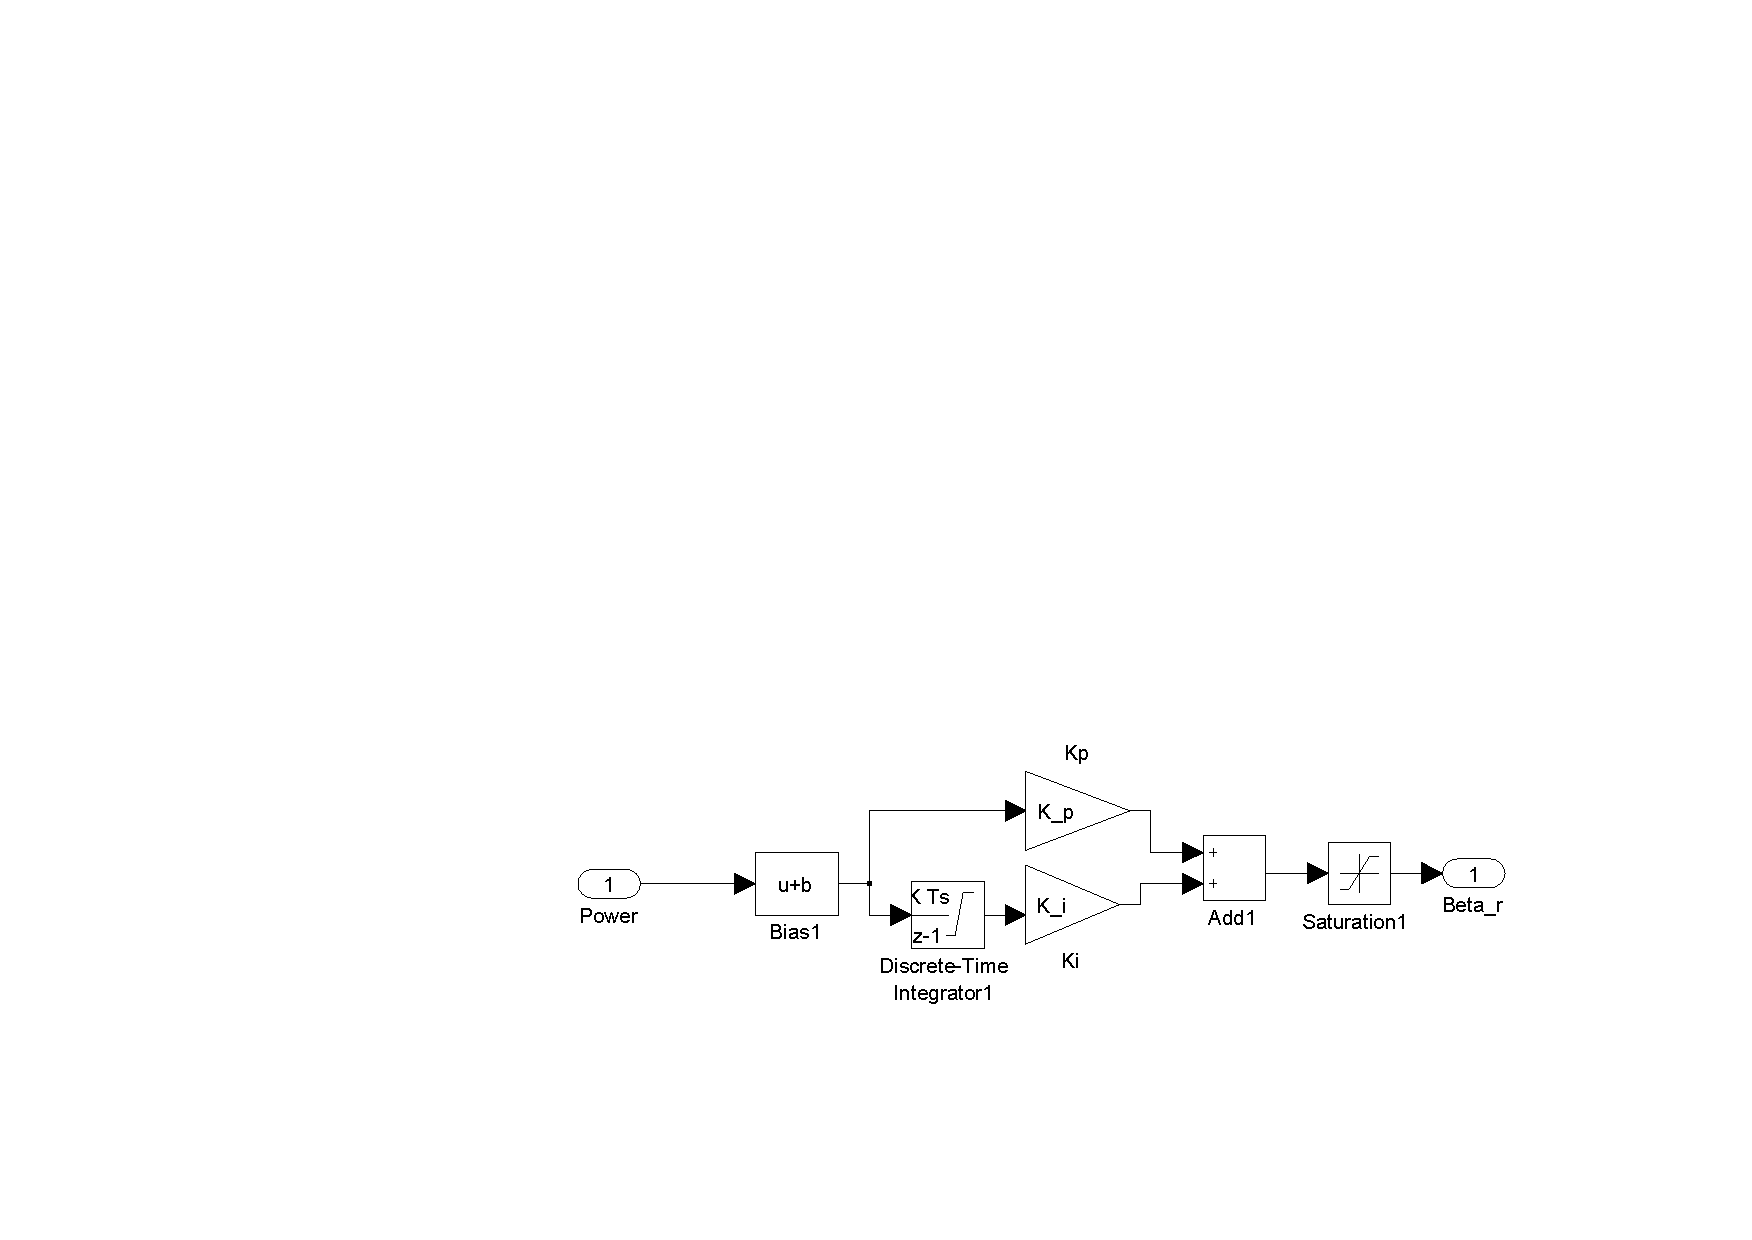
\includegraphics[width=\hsize]{MATLAB_PI.pdf}
  \caption{Simulation Model of PI Controller}
  \label{fig:pi_controller}
\end{figure}

The wind data is downloaded from the kk-electronics project\cite{ref:kke}, and is depicted in Fig.\ref{fig:wind}. Simulation results are shown in Fig.\ref{fig:pumpwear} to Fig.\ref{fig:highair} where the fault diagnosis result of pump wear fault, hydraulic leakage fault and high air content fault. The forgetting factor is chosen to be $0.97$ according to Eq.\ref{e:f}, and fault indicator of three situations are the same:

\begin{equation}
  \alpha_{pw},\alpha_{hl},\alpha_{ha}=
  \begin{cases}
    0, & 0\leq{}t\leq1000, 2000\leq{}t\leq3000 \\
    1, & 1000 <t< 2000, 3000 <t< 4500
  \end{cases}
\end{equation}

Results of Fig.\ref{fig:pumpwear} to Fig.\ref{fig:highair} show that when the innovation length gets larger, the algorithm will have a faster convergence. And when simulation begins, the $p=1$ algorithm fails to track the parameter.

\begin{figure}[!htb]
\centering
  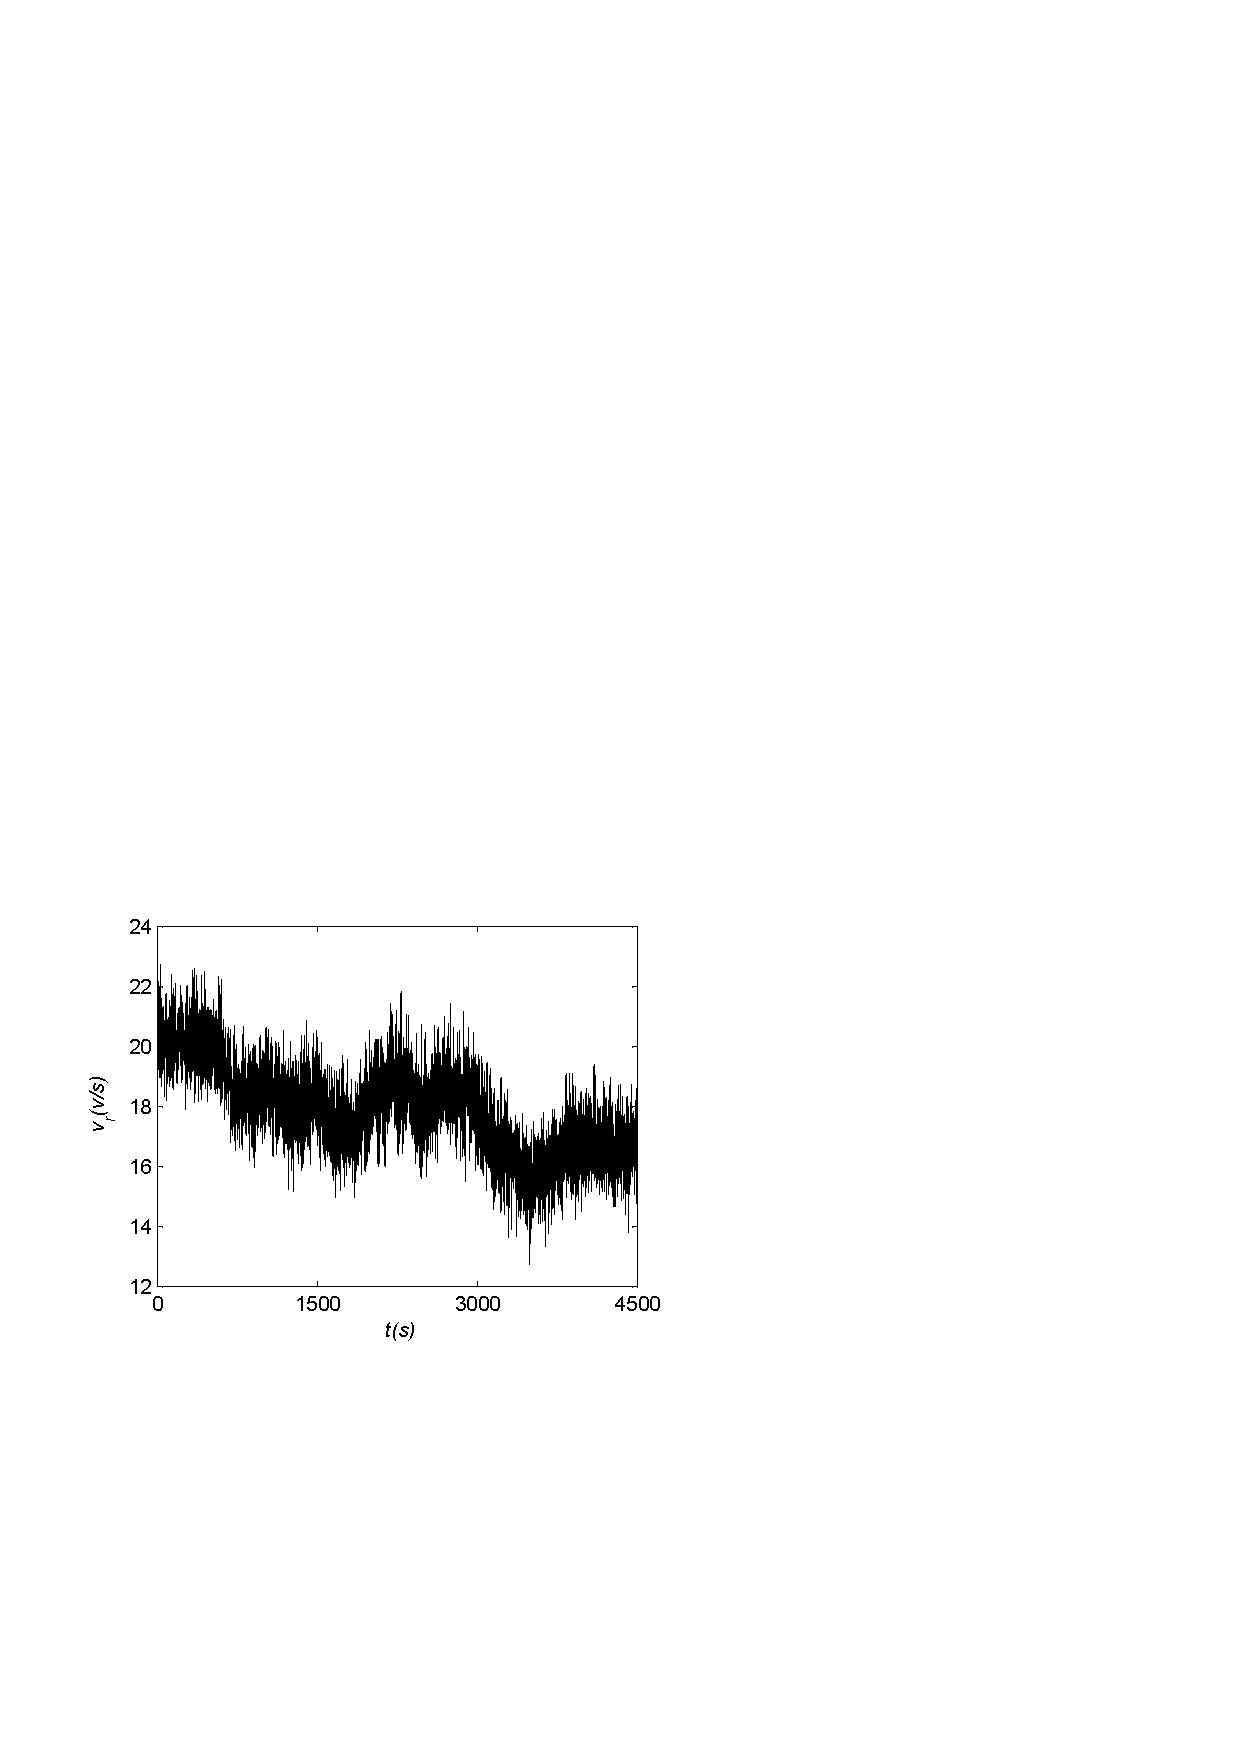
\includegraphics[]{MATLAB_wind.pdf}
  \caption{Wind Velocity}
  \label{fig:wind}
\end{figure}

\begin{figure}[!htb]
\centering
  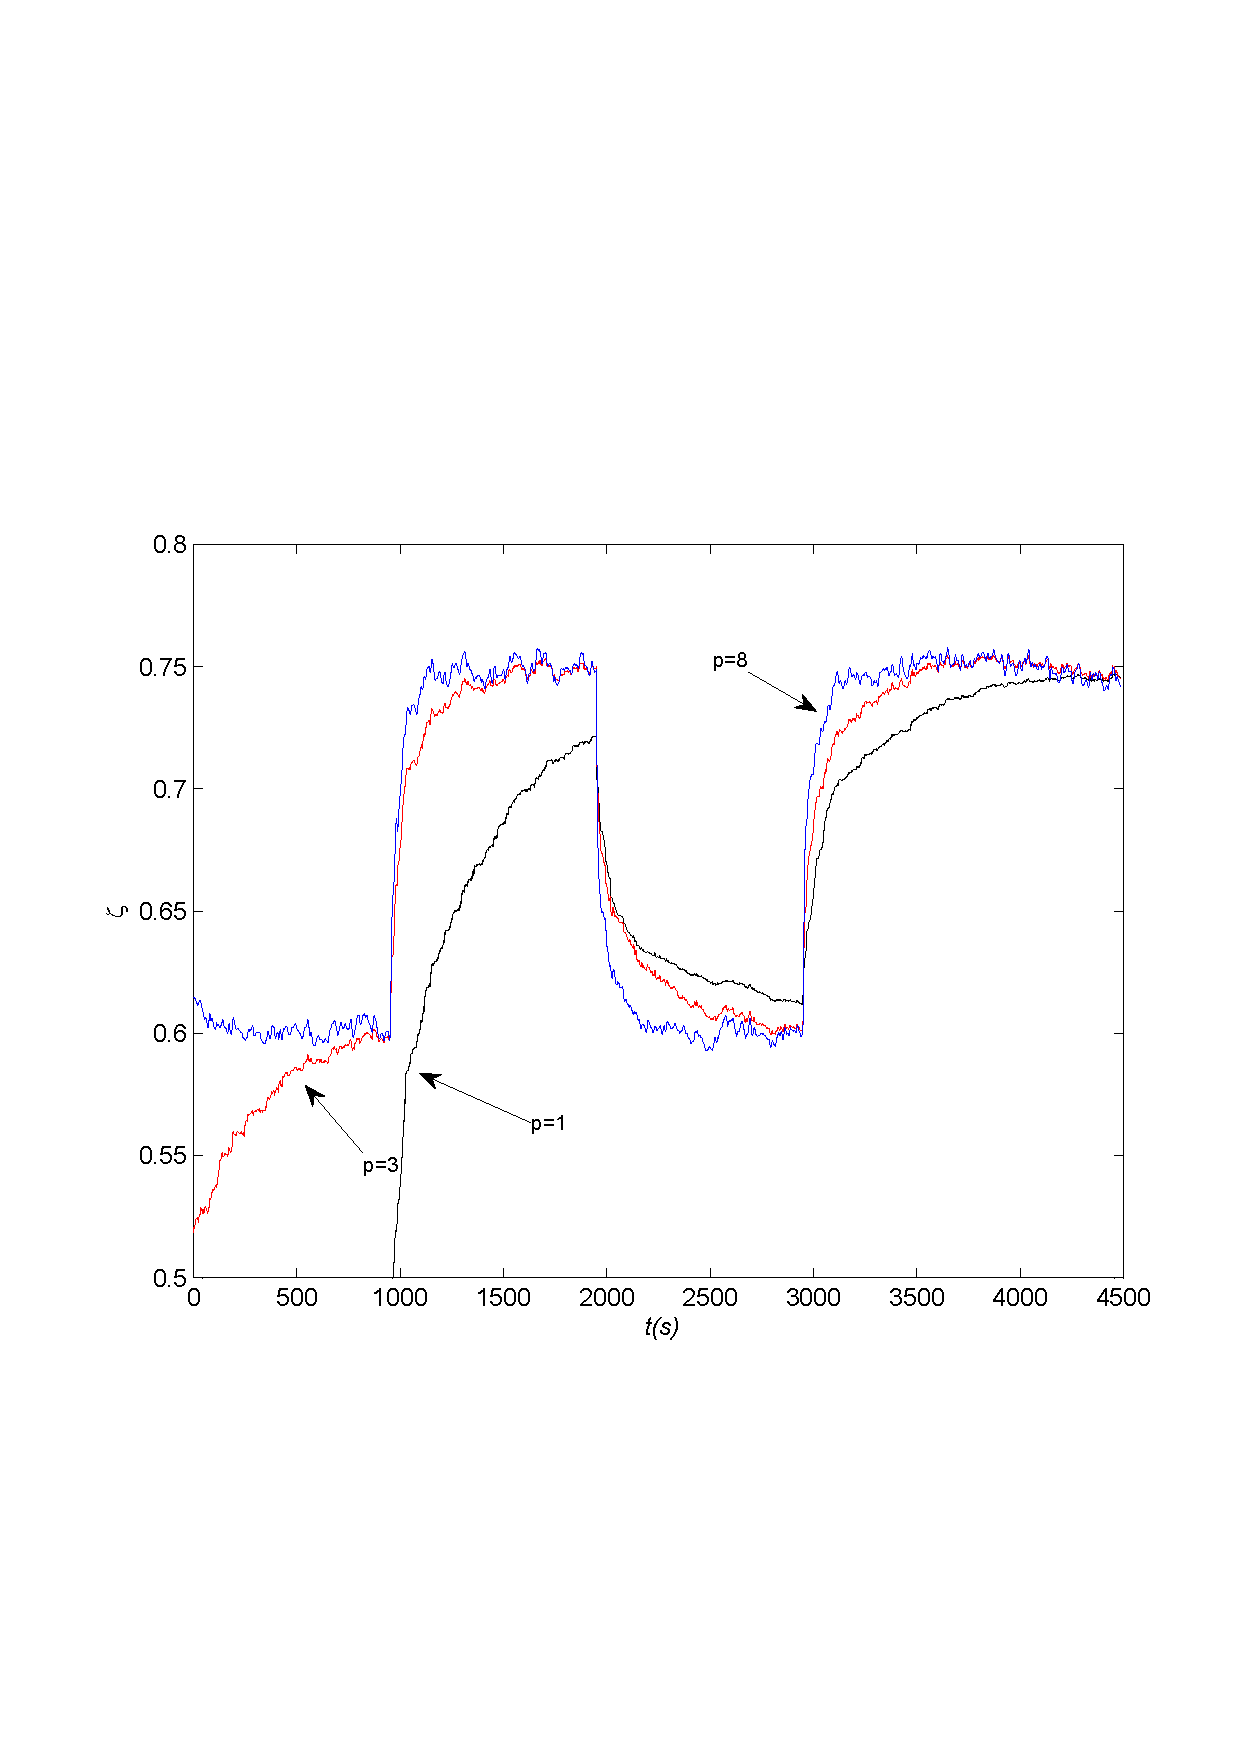
\includegraphics[scale=0.5]{MATLAB_zeta075.pdf}
  \caption{$\zeta$ with Pump Wear Fault}
  \label{fig:pumpwear}
\end{figure}

\begin{figure}[!htb]
\centering
  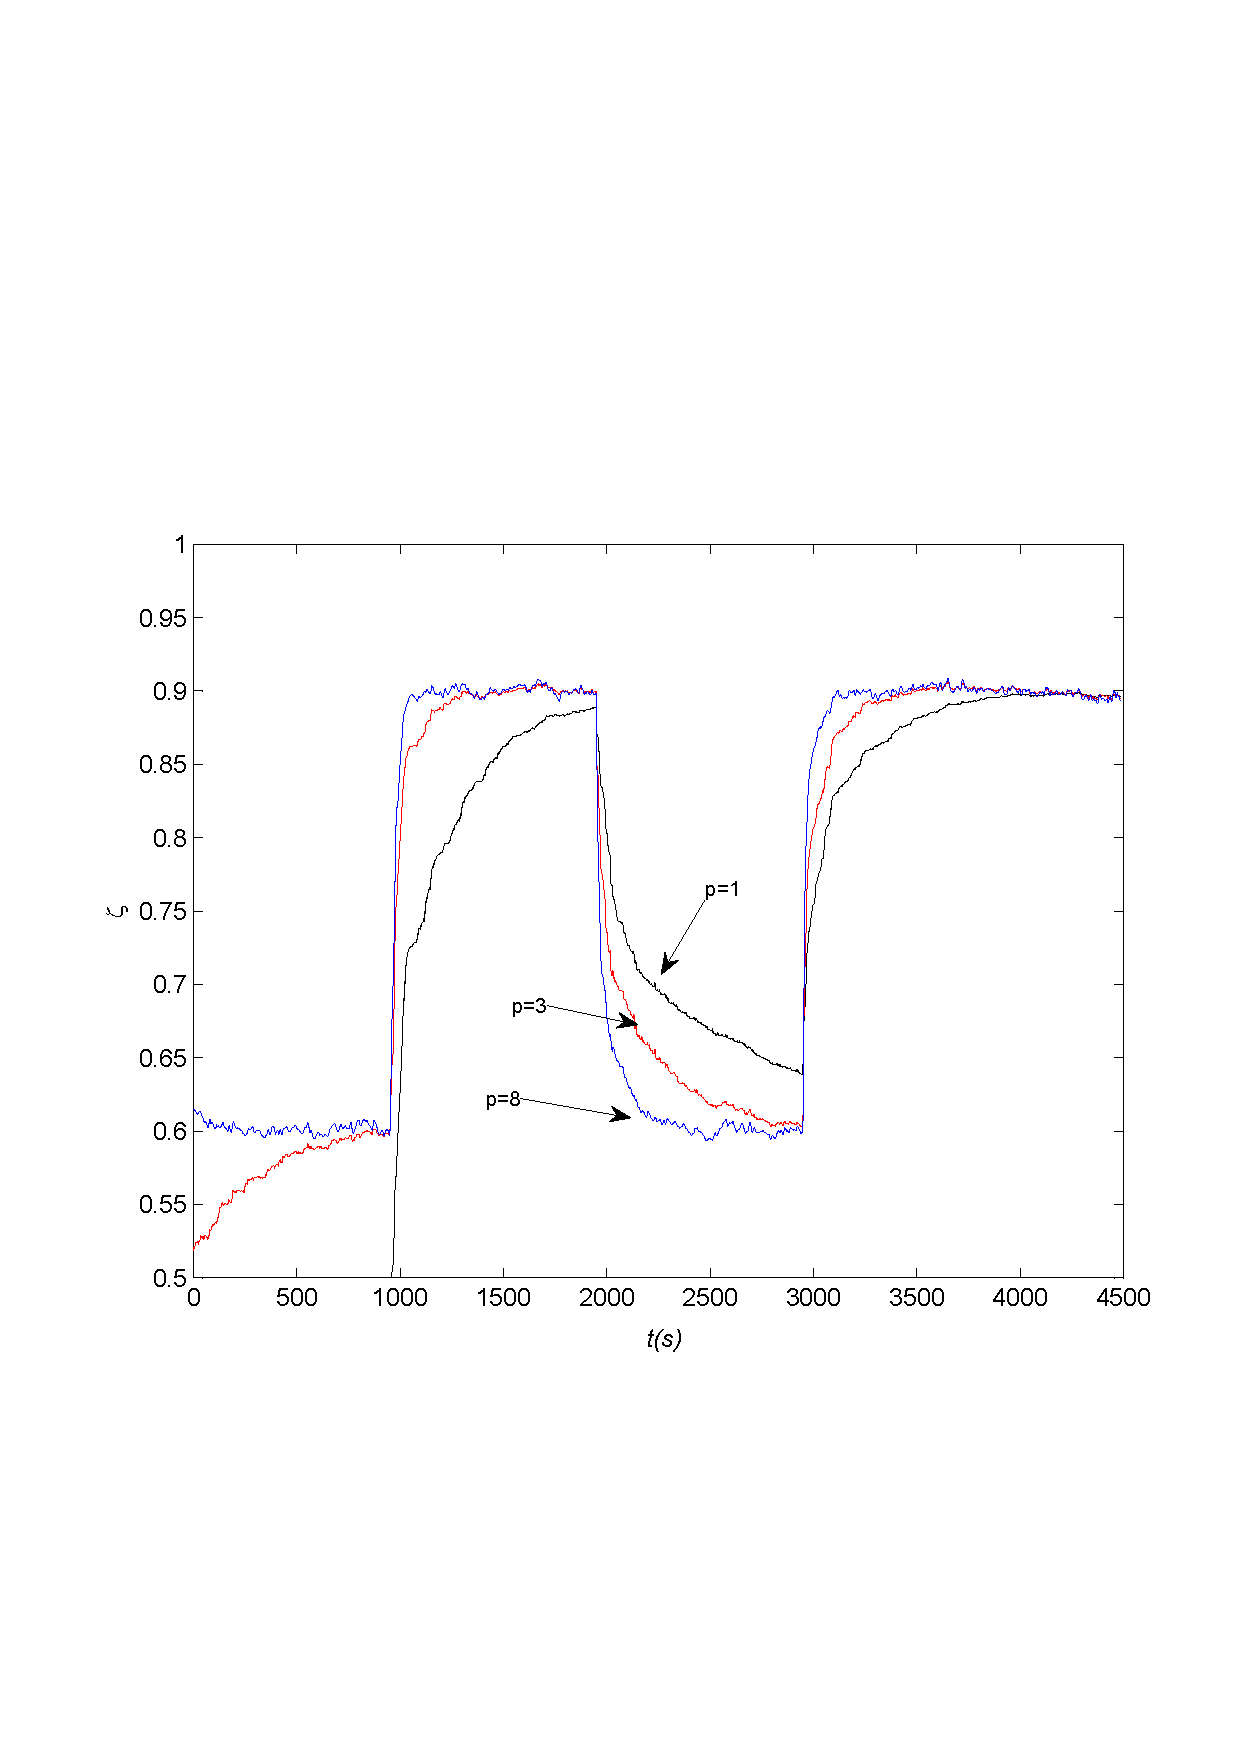
\includegraphics[scale=0.5]{MATLAB_zeta09.pdf}
  \caption{$\zeta$ with Hydraulic Leakage Fault}
  \label{fig:leakage}
\end{figure}

\begin{figure}[!htb]
\centering
  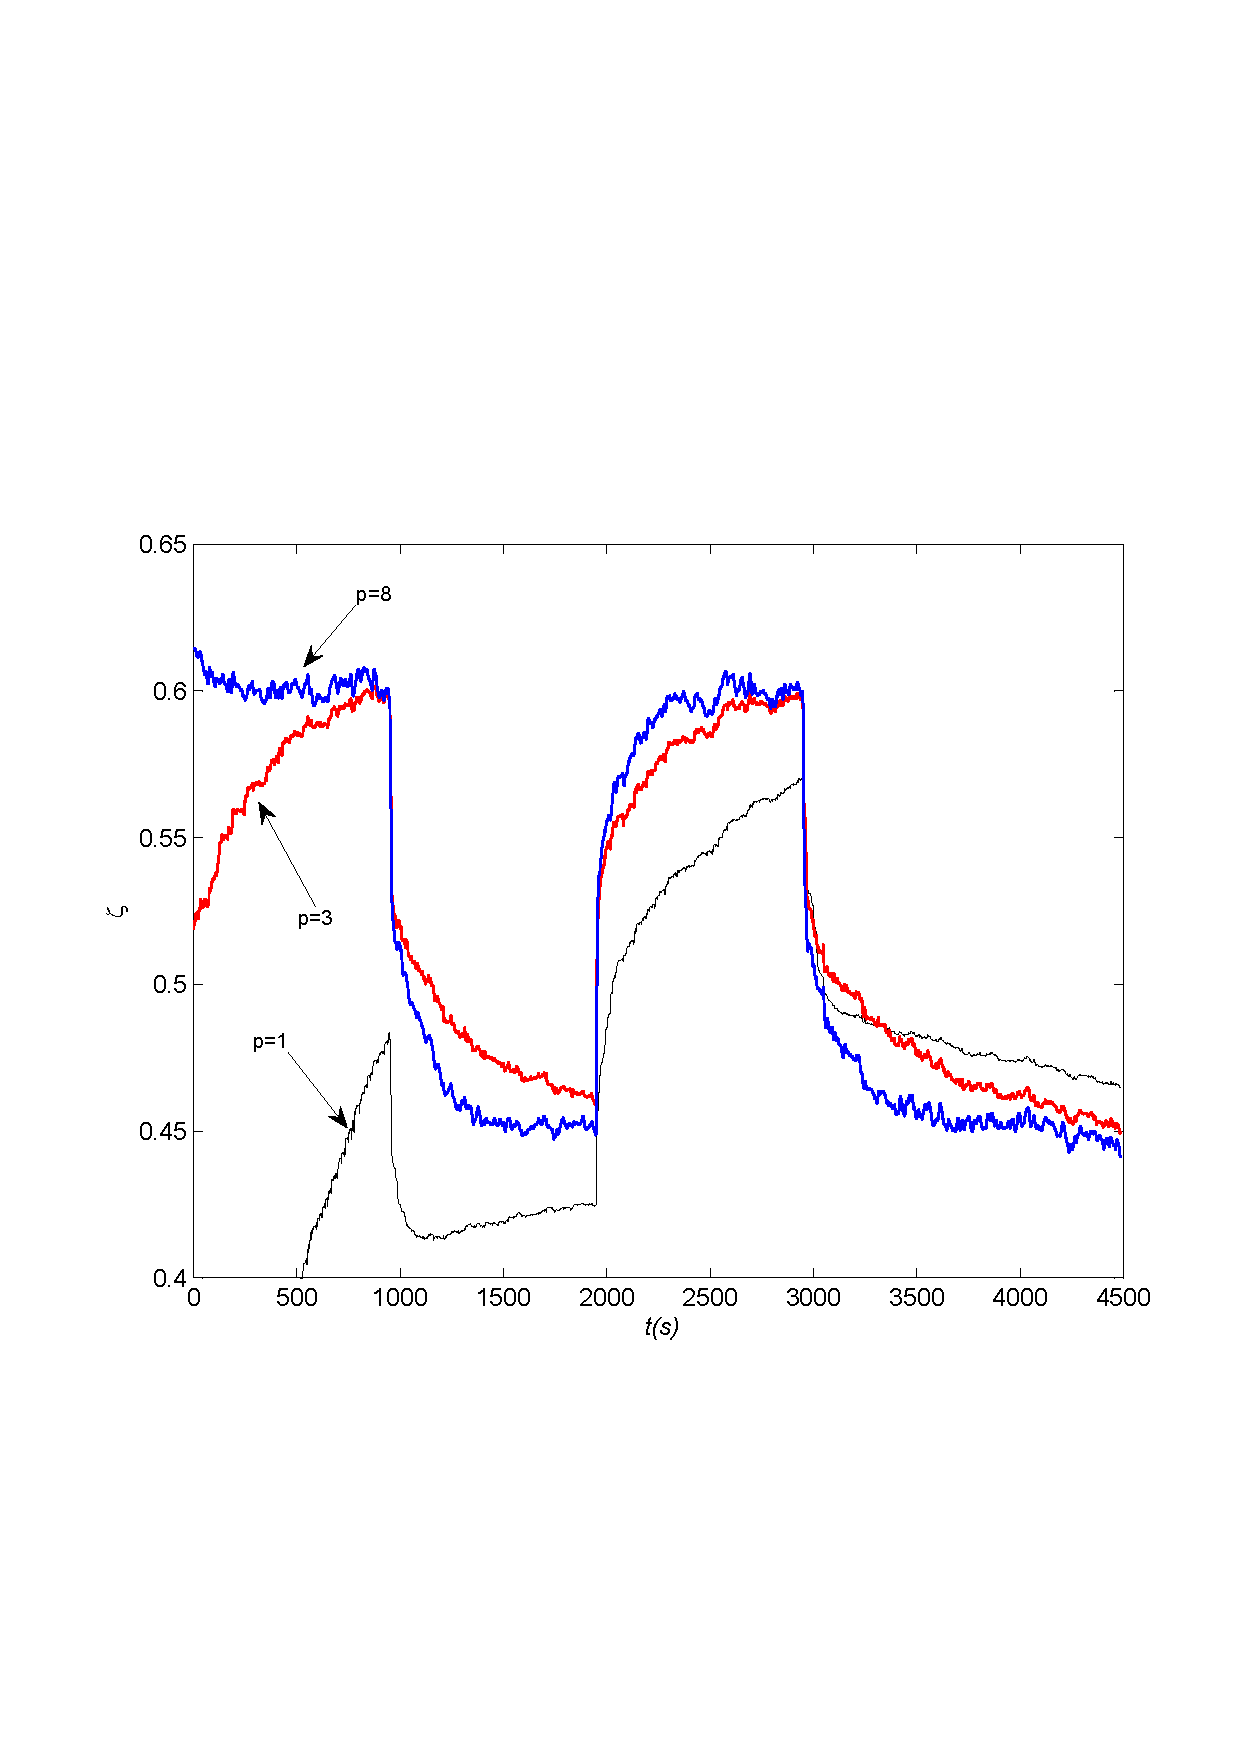
\includegraphics[scale=0.5]{MATLAB_zeta045.pdf}
  \caption{$\zeta$ with High Air Content Fault}
  \label{fig:highair}
\end{figure}

We also test the real simulation time, the time is shown in Tab.\ref{tab:time}. As the innovation length gets larger, it takes more computation time as the matrix becomes more complex. As the Tab.\ref{tab:time} suggests, innovation length $p=8$ is better.

\begin{table}[!htb]
  \centering
  \caption{Real Simulation Time} \label{tab:time}
\begin{tabular}{|c|c|}
  \hline
  % after \\: \hline or \cline{col1-col2} \cline{col3-col4} ...
  Innovation length & Time \\\hline\hline
    $p=1$     &   $0.313650s$ \\\hline
    $p=3$         & $0.270484s$ \\\hline
    $p=8$         & $0.360650s$ \\\hline
    $p=12$         & $0.497493s$ \\\hline
    $p=14$         & $0.534856s$ \\\hline
    $p=16$         & $0.601536s$ \\\hline
    $p=32$         & $0.894214s$ \\\hline
  \hline
\end{tabular}
\end{table}


\section{Conclusion}

In this paper, we convert the fault diagnosis problem into a system identification issue, which means that changed parameter can reflect what kind of fault. The variable pitch system of wind turbine can be modeled as a second order system. Analysis of how to choose forgetting factor and innovation length is given in detail. A larger innovation length and a appropriate forgetting factor will produce a smaller estimation error and faster convergence. The simulation results verify the validity of the analysis.


\section*{Funding}

This research was supported by Prospective Joint Research Project of Industry, Education and Academy of Jiangsu Province(BY2012071) and China Postdoctoral Science Foundation (2013M531272).



\begin{thebibliography}{0}
\bibitem{ref:1}
Global Wind Energy Council. Global wind report -- annual market
update 2011. Brussels Belgium: Global Wind Energy Council,
2012.

\bibitem{ref:2}
Dobrila O, Stefansen R. \emph{Fault tolerant wind turbine control}.
Denmark: Technical  University  of  Denmark, 2007.

\bibitem{ref:3}
Li SB, Sauter D, Aubrun C. Stability guaranteed active fault-tolerant control of networked control systems . \emph{Journal of Control Science and Engineering}. 2008; 5: 22 -- 31.

\bibitem{ref:wind zone}
Bianchi FD, Battista HD, Mantz RJ. Wind Turbine Control Systems �C Principle, Modelling and Gain Scheduling Design.
\emph{London: Springer}, 2007:18 -- 19.

\bibitem{ref:neural BP}
Wang SP, Wang ZL. The neural network method of hydraulic pump fault
diagnosis. \emph{Journal of Beijing University of Aeronautics and
Astronautics}, 1997; 23(6): 714 -- 718.

\bibitem{ref:qualitative pitch}
Goharrizi AY, Sepehri N. A wavelet-based approach to internal seal damage diagnosis in hydraulic actuators. \emph{IEEE Transactions on Industrial Electronics}, 2010; 57(5): 1755--1763.

\bibitem{ref:active LPV}
Esbensen T, Sloth C.
 \emph{Fault Diagnosis and Fault-Tolerant Control of Wind Turbines}.
 Aalborg University, 2009; 16--21, 100--104.

%%%%%%%%%%%%%%%%%%%%%%%
%% 2013.9.27 begin
%%%%%%%%%%%%%%%%%%%%%%%
\bibitem{ref:ding1}
Ljung L. \emph{System identification: Theory for the user}. Prentice-Hall: Englewood Cliffs, NJ, 1999.

\bibitem{ref:ding2}
Ding F, Chen T. Modeling and identification for multirate systems. \emph{Acta Automatica Sinica}, 2005; 31(1): 105 -- 122

\bibitem{ref:ding3}
Ding F, Lin P, Liu G. Auxiliary model based multi-innovation extended stochastic gradient parameter estimation with colored measurement noises. \emph{Signal Processing}, 2009; 89(10): 1883 -- 1890.

\bibitem{ref:ding4}
Ding F, Chen T. Hierachical least squares identifiaction methods for multivariable systems. \emph{IEEE Transactions on Automatic Control}, 2005; 50(3): 397 -- 402.
%%%%%%%%%%%%%%%%%%%%%%%
%% 2013.9.27 end
%%%%%%%%%%%%%%%%%%%%%%%

\bibitem{ref:rls}
Guo L, Ljung L. Exponential stability of general tracking algorithms. \emph{IEEE Transactions on Automatic Control}. 1995; 40(8): 1376 -- 1387.

\bibitem{ref:rffls}
Guo L, Ljung L. Performance analysis of general tracking algorithms. \emph{IEEE Transactions on Automatic Control}. 1995; 40(8): 1388 -- 1402.

\bibitem{ref:misg}
Ding F, Chen T. Performance bounds of forgetting factor least
squares algorithm for time-varying systems with finite measurement data.
\emph{IEEE Transactions on Circuits and Systems��I: Regular Papers}, 2005; 52(3):
555 -- 566.


%%%%%%%%%%%%%%%%%%%%%%%
%% 2013.9.27 begin
%%%%%%%%%%%%%%%%%%%%%%%
\bibitem{ref:lyy1}
Spera DA. \emph{Wind turbine technology}. 1994.

\bibitem{ref:robust1}
Muljadi E, Butterfield CP. Pitch-controlled variable-speed wind turbine generation. \emph{IEEE Transactions on Industry Applications}, 2001; 37(1): 240 -- 246.

\bibitem{ref:robust2}
Muyeen SM, Ali MH, Takahashi R, et al. Comparative study on transient stability analysis of wind turbine generator system using different drive train models. \emph{Renewable Power Generation}, 2007; 1(2): 131 -- 141.

\bibitem{ref:ding5}
Ding F. System identification. Part B: Basic models for system description. \emph{Journal of Nanjing University of Information Science and Technology: Natural Science Edition}, 2011; 3(2): 97 -- 117.

\bibitem{ref:dinf6}
Ding F, Chen HB, Li M. Multi-innvation least squares identification methods based on the auxiliaty model for MISO systems. \emph{Applied Mathematics and Computation}, 2007; 187(2): 658 -- 668.

\bibitem{ref:kke}
kk-electronic a/s. Fault tolerant control of wind turbines a benchmark model.
http://www.kk-electronic.dk/Default.aspx?ID=9338/(2010).
%%%%%%%%%%%%%%%%%%%%%%%
%% 2013.9.27 end
%%%%%%%%%%%%%%%%%%%%%%%
\end{thebibliography}



\end{document} 